% Manuscript in the CVPR 2026 author-kit format.
% Eight-page main-track budget. Not a submission.
\documentclass[10pt,twocolumn,letterpaper]{article}
\usepackage{cvpr}
\usepackage{fontspec}
\setmainfont{Times New Roman}
\setsansfont{Helvetica}
\setmonofont{Courier New}
\usepackage{graphicx}
\usepackage{booktabs}
\usepackage{amsmath}
\usepackage{amssymb}
\usepackage{amsthm}
\newtheorem{theorem}{Theorem}
\newtheorem{proposition}{Proposition}
\definecolor{cvprblue}{rgb}{0.21,0.49,0.74}
\usepackage[pagebackref,breaklinks,colorlinks,allcolors=cvprblue]{hyperref}

\def\paperID{*****}
\def\confName{CVPR}
\def\confYear{2026}

\title{Imputation Decides:\\The Measured Cost of Filling Unobserved Input}

\author{Worldtick\\
{\tt\small https://github.com/shaneraphel/aletheia-worldtick}
}

\begin{document}
\maketitle

\begin{abstract}
World models, neural decoders, and action models share one inference step: impute what was not observed, then decide from the completed input.
We measure that step in three settings that compile to integers: occupancy reachability, EEG classification, and tabular action selection.
Optimistic imputation returns the number a fully observed input would have returned.
A single measured transition returns a smaller number, and empty input raises rather than returning zero.
On 10{,}000 corridors, imputation walks into an occluded obstacle 2{,}995 times and a measured step does so 0 times.
On 2{,}000 grids of $16{\times}16$, a selector that prefers the shorter imagined path reaches the goal 500 times and crashes 1{,}439 times, while an oracle choosing among the same two plans reaches 797 times.
The gap is selection.
A closed form gives the discount at which lookahead flips a trap, $9/101$, and finite-horizon dynamic programming matches the infinite horizon at depth one on 1{,}000 random traps.
Re-observing before every step removes the 2{,}995 collisions.
Every count is recomputed from a pinned seed and checked against the manuscript.
\end{abstract}

\section{Introduction}
\label{sec:intro}

A planner that cannot see a cell still has to say whether that cell is free.
The 2026 default is to fill the cell in.
Video world models predict masked patches~\cite{vjepa21,vjepa2}.
Reconstruction latents, including Cosmos-style tokenizers, are trained so the filled frame matches pixels~\cite{nilaksh2026}.
Large EEG models predict masked neural patches, and missing channels are interpolated onto the pretraining montage~\cite{jiang2024labram}.
World action models render a future and then read an action off that rendering~\cite{visual2026,wcd2026}.

Two results from 2026 say that this default is not the decision.
Nilaksh~\etal show that pixel fidelity does not select the latent space that plans well: reconstruction encoders win image metrics, and semantic encoders win policy behavior~\cite{nilaksh2026}.
A study of test-time planning with world action models finds that an oracle, which picks the sampled future whose realized outcome is best, lifts success from $68.9\%$ to $79.2\%$, while selectors based on visual quality recover little of that gap~\cite{visual2026}.
Both papers evaluate learned models on robot benchmarks.
What they do not provide is a setting in which the imputed value, the measured value, and the selector gap are exact integers that a reviewer can recompute.

This paper builds that setting.
The claim is narrow.
Where an unobserved cell is written as a usable value, the written value decides the failure mode.
We do not re-run the published robot success rates.
We re-run the shared step: write a number into a place that was not seen, then compare it with a transition that uses only an observed fact.

\begin{figure}[t]
  \centering
  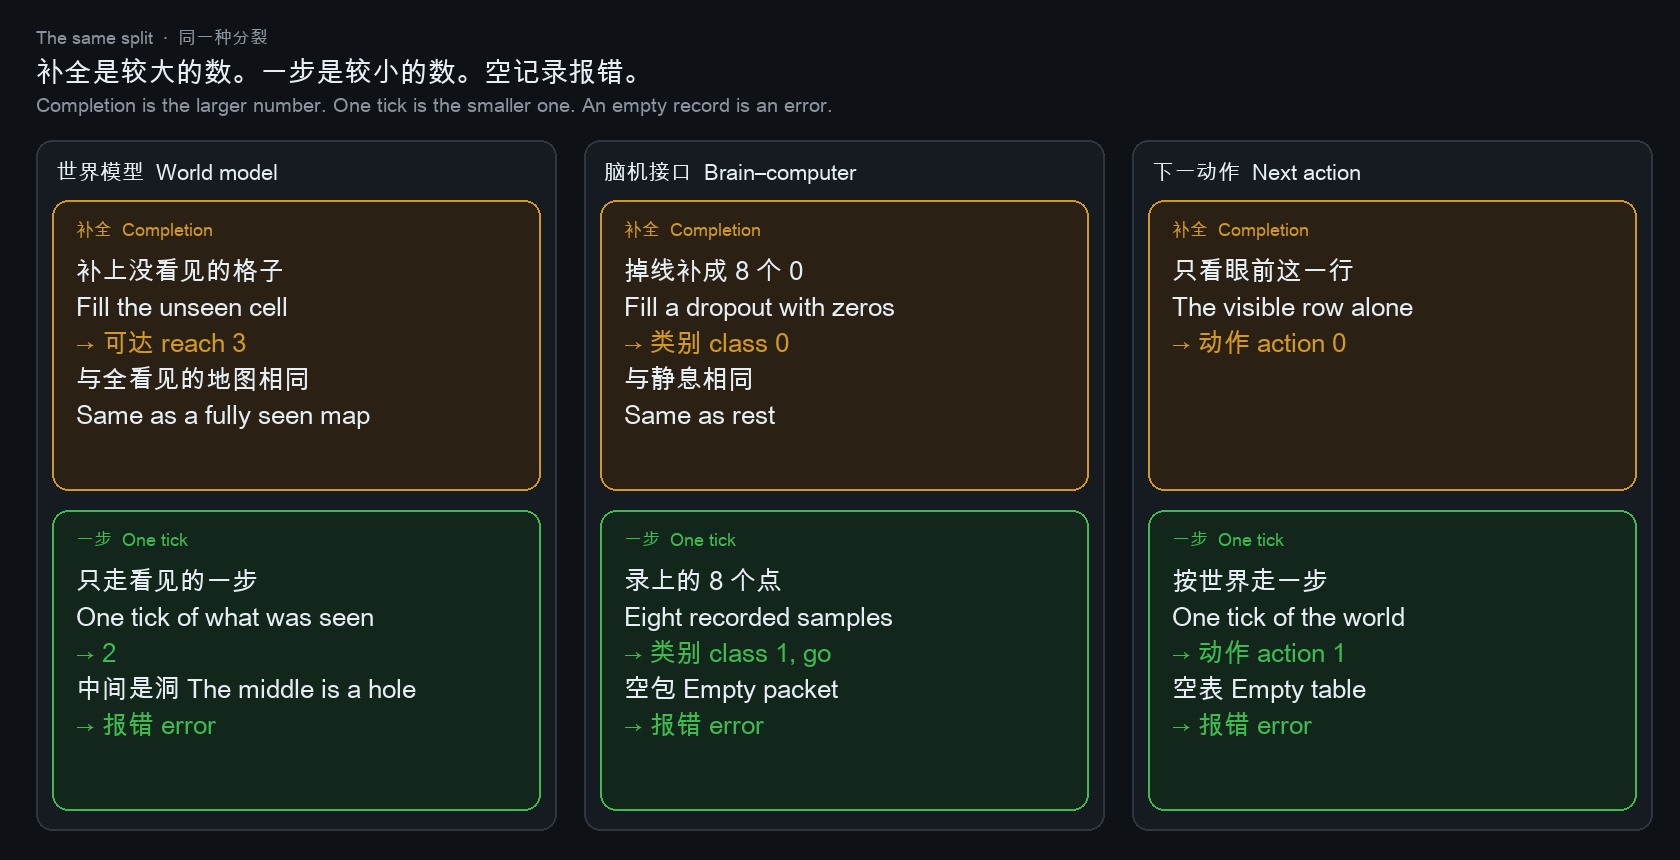
\includegraphics[width=\linewidth]{../../docs/figures/story.png}
  \caption{One split, three fields. Imputation returns the larger integer. One measured step returns the smaller integer. Empty input raises.}
  \label{fig:story}
\end{figure}

\section{Related work}

\paragraph{World models.}
Joint-embedding predictors learn by predicting held-out video tokens from visible context~\cite{vjepa2,vjepa21}.
Action-conditioned variants roll those predictions forward and plan toward image goals.
The reconstruction-or-semantics study trains latent diffusion world models on BridgeV2 under a fixed protocol and finds that visual scores and planning scores disagree~\cite{nilaksh2026}.
Our occupancy experiments isolate that disagreement from the generator: the same shortest-path routine is run on an imputed grid and on observed cells.

\paragraph{Neural decoding.}
LaBraM pretrains a transformer by predicting quantized codes of masked EEG patches~\cite{jiang2024labram}.
Deploying the checkpoint on a different montage requires a spatial interpolation layer so the backbone sees its canonical channels.
Zero-filling a dropped packet is the trivial form of that step.
We measure when the filled packet is classified as rest.

\paragraph{Test-time selection.}
World action models sample futures and rank them~\cite{visual2026,wcd2026}.
The published finding is that ranking by how the future looks is not ranking by whether the action succeeds.
Section~\ref{sec:selector} measures the same split on grids, with an oracle that sees the true obstacles and a visual score that sees only path length on the imputed map.

\section{Operators}
\label{sec:ops}

An observation is a grid, a sample vector, or a reward table, with a subset of entries marked missing.
Three operators are applied to the same observation.

\paragraph{Optimistic imputation.}
Missing map cells are written free.
A dropped EEG suffix is written as zeros.
The next action is the maximum of the visible reward row.
The operator returns a completed object on which an ordinary algorithm runs: a fixed-point reachable set, a sum classifier, or one Bellman backup.

\paragraph{Measured step.}
Only entries that were observed are used.
On a chain, occupied facts move across one edge.
On a grid, masked cells are treated as blocked.
On EEG, an empty vector raises.
On a reward table, the action is the optimum of a finite-horizon backup, not of the raw row.

\paragraph{Pessimistic fill.}
Missing cells are written as obstacles.
Every cell the resulting path enters was observed free, so the path cannot cross an occluded obstacle.

Empty input is fail-closed for each operator that would otherwise return a zero, an empty list, or a not-a-number.
The occupied input keeps its value: a $2{\times}2$ assignment stays cost $2$, eight recorded EEG samples stay class $1$, and two lidar returns stay a count of $1$.

\section{Theorems}

\begin{theorem}[Foresight threshold]
On the reward table $[[10,1],[-100,-100]]$, with the ring transition $(s+a+1)\bmod 2$, the optimal action at state $0$ flips from $0$ to $1$ at discount $d=9/101$.
\end{theorem}
\begin{proof}
Under the stationary policy ``always action $0$'', the state values satisfy $V_0=10+dV_1$ and $V_1=-100+dV_0$, so $V_0=(10-100d)/(1-d^2)$.
The one-step alternative at state $0$ is $Q_0(a_1)=1+dV_0$.
Then $Q_0(a_1)>V_0$ if and only if $1+d>10-100d$, that is $101d>9$.
Policy evaluation solves $(I-dP)V=r$ in exact rationals, so the inequality is sharp on the grid $d\in\{0.00,\ldots,0.08\}$ (action $0$) and $d\in\{0.09,\ldots,0.95\}$ (action $1$).
\end{proof}

\begin{theorem}[Mask erasure]
Optimistic imputation emits no mask marker.
Any checker that tests for a missing-data flag has recall $0$ on imputed maps.
\end{theorem}
\begin{proof}
The fill replaces each missing entry by $0$ or by a wall bit.
The output domain is the fully observed domain.
On 10{,}000 corridors the count of surviving markers is $0$, while 8{,}564 of those maps still hide an obstacle.
\end{proof}

\begin{theorem}[Monotone convergence]
Reachability from a fixed observed set, iterated one edge at a time, is nondecreasing and bounded by the fixed point, hence convergent.
\end{theorem}
On the pinned world (256 nodes, 8 observed facts, 512 edges, seed 20260919) the sequence is $8,24,50,92,138,205,212,214$ and meets the fixed point at horizon $12$.

\begin{proposition}[Pessimistic safety]
A path that treats missing cells as blocked never enters an occluded obstacle.
\end{proposition}
Every entered cell was observed free.
On 10{,}000 corridors the collision count is $0$.
The price is $10{,}000$ early stops and $0$ completed traversals when the fill is used as an open-loop plan.

\begin{theorem}[Breakeven]
Let $C$ be the number of crashes under optimistic imputation and $W$ the number of waits under the measured policy on the same corridors.
The measured policy has lower total cost if and only if one crash costs more than $W/C$ waits.
\end{theorem}
\begin{proof}
Both costs are linear in the crash price $c$.
Equality holds at $c=W/C$.
The pinned counts give $W/C=2353/552$ for one-step decisions and $W/C=20975/2995$ for full-corridor walks.
\end{proof}

\section{Experiments}
\label{sec:exp}

All trials use seed 20260919 unless a seed list is stated.
Counts are written to JSON and checked against this manuscript by a script in the repository.
Wilson intervals below are closed form on those counts.
They are not a second sample.

\subsection{Three fields, one pair of integers}

Figure~\ref{fig:story} is the unit case.
A three-cell chain with the middle cell missing reaches $3$ after imputation and $2$ after one measured step.
An eight-sample EEG packet that sums positive is class $1$; the same length filled with zeros is class $0$, identical to rest.
On the trap table the visible row selects action $0$ and one-step lookahead selects action $1$.
Empty input raises in each field.

The same pair appears at larger width.
On 10{,}000 chains of eight cells, imputation reaches $8$ and the measured step reaches $2$ in every trial.
Zero-filled EEG packets match rest in every trial, and the myopic action differs from lookahead in every trial.

\subsection{Corridors}

A corridor is a line of $32$ cells.
Each cell after the start is an obstacle with probability $0.20$ and is masked with probability $0.30$.
Optimistic imputation writes masked cells free and walks until it hits an observed obstacle or a true obstacle that was written free.
The measured step stops at the first mask.

Of 10{,}000 corridors, 8{,}564 contain an occluded obstacle.
Imputation enters one on 2{,}995 corridors.
The measured step enters one on $0$ corridors.
A next-cell decision on the same distribution collides 552 times under imputation and $0$ times under the measured step, which instead stops on 2{,}353 free roads.
Varying only the mask rate from $0$ to $0.50$, with 10{,}000 corridors at each of seven rates, imputation entries are $0,503,934,2002,2914,3970,5084$.
The measured step stays at $0$.

Pessimistic fill, which writes masks as walls, records $0$ collisions, $10{,}000$ stops, and $0$ completed walks.
Optimistic fill on the same roads records 2{,}995 collisions, 6{,}993 stops, and 12 completed walks.
The planner is held fixed.
The fill is the variable.

Re-observing the next cell before every step, and waiting when the look is masked, records $0$ collisions, $9$ completed walks, $9{,}991$ stops at an observed obstacle, and $20{,}975$ waits.
Open-loop optimism on the comparable full walk collides 2{,}995 times.
Figure~\ref{fig:loop} puts the two policies on one plot.
The closed loop reaches the end $9$ times, against $12$ for open-loop optimism, and it stops at an observed obstacle $9{,}991$ times.
The waits, $20{,}975$ in total, are the price of not writing the mask as free.
By Theorem~5 that price is the cheaper side whenever one collision costs more than $20975/2995\approx 7$ waits.

\begin{figure}[t]
  \centering
  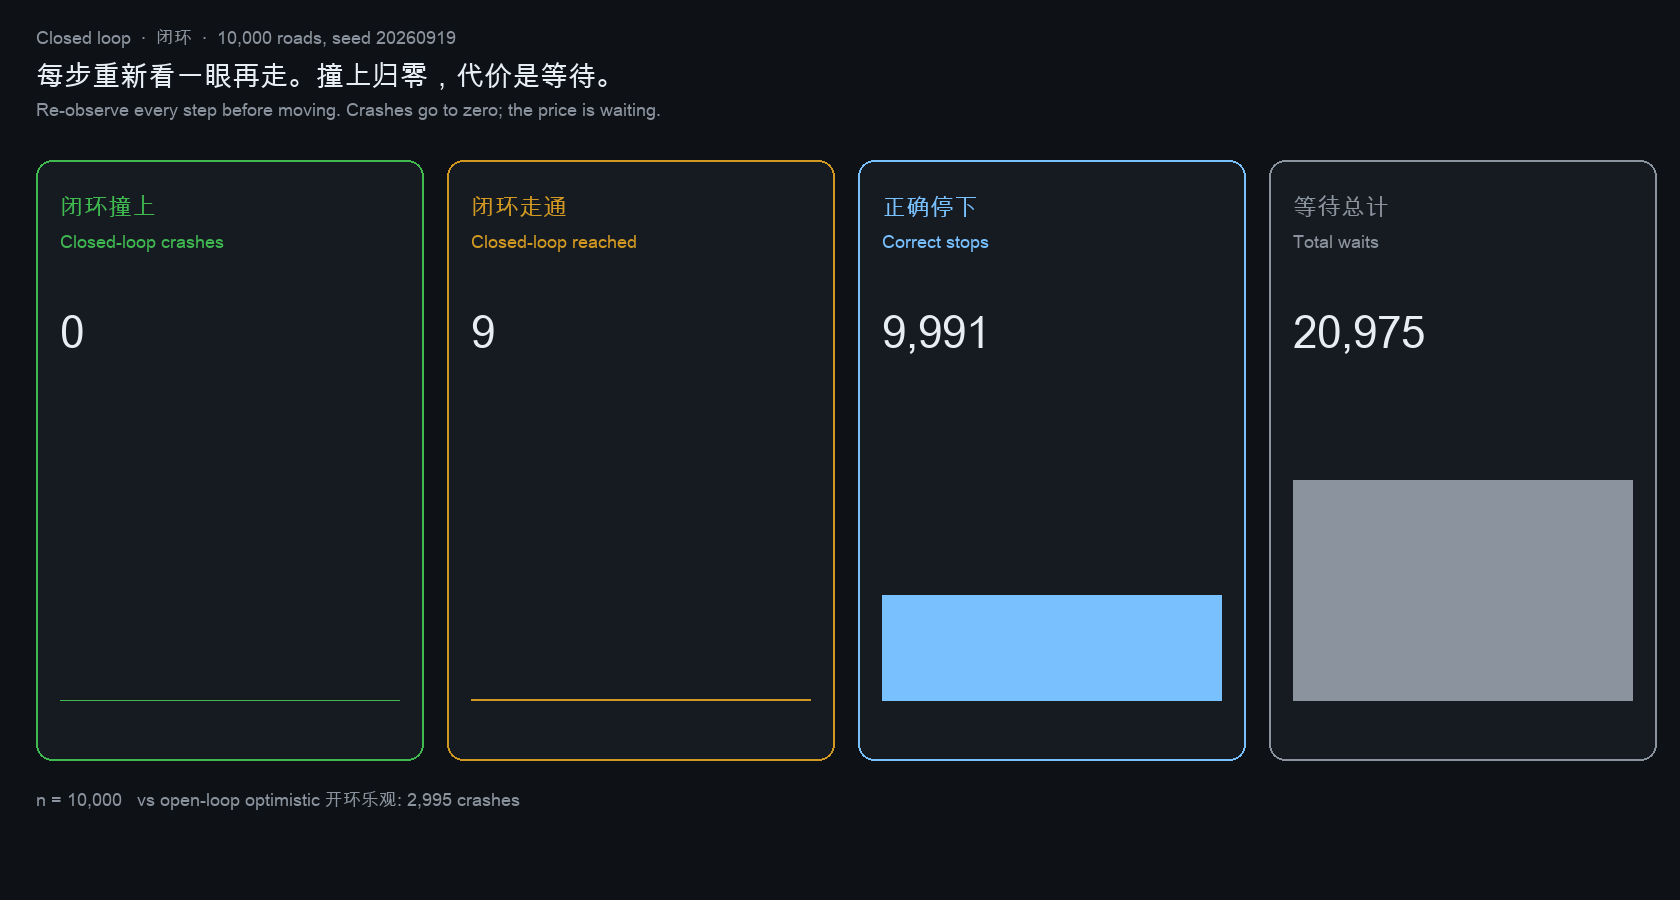
\includegraphics[width=\linewidth]{../../docs/figures/closedloop.png}
  \caption{Re-observing before each step. Crashes are $0$, against $2{,}995$ for open-loop optimistic imputation. The price is $20{,}975$ waits.}
  \label{fig:loop}
\end{figure}

\subsection{Horizon and its cost}

On the pinned 256-node world, reach after $h$ steps is $8,24,50,92,138,205,212$ and $214$ at $h=12$, then flat through $h=256$.
One call to the fixed-point operator returns $214$.
Median call time grows with $h$ and flattens at the same index.
On the reference machine a single fixed-point call is about $0.09$\,ms.
Timings are reported, not pinned.

\subsection{Foresight and depth}

The trap proof is checked on a discount grid.
Actions are $0$ for $d\le 0.08$ and $1$ for $d\ge 0.09$.
One thousand random traps, with the same sign pattern and randomized magnitudes, all flip between $d=0$ and $d=0.9$.

Finite-horizon dynamic programming at discount $9/10$ tells how many backups are required.
Depth $0$ is the myopic row and flips $0$ of 1{,}000 tables.
Depths $1$ through $5$ flip $1{,}000$ of $1{,}000$ and match the infinite-horizon optimum on every table.
On a one-step trap, one backup is the horizon.
The fixed trap by depth is $0,1,1,1,1,1$.

\subsection{EEG dose--response}

Ten thousand random packets of eight samples, conditioned to be class go, have a suffix of length $k$ replaced by zeros.
Packets then classified as rest, for $k=0,\ldots,8$, number $0,0,1,9,43,161,642,2494,10000$.
Dropping the whole packet makes every go trial indistinguishable from rest.
An empty vector, which is not a zero-filled vector, raises.
Figure~\ref{fig:eeg} plots the dose.
The rise is slow through four dropped samples (43 of 10{,}000) and then steep: 2{,}494 at seven dropped samples, and 10{,}000 when the packet is entirely zeros.
A decoder that never sees a mask bit cannot tell the last of these from a subject at rest.

\begin{figure}[t]
  \centering
  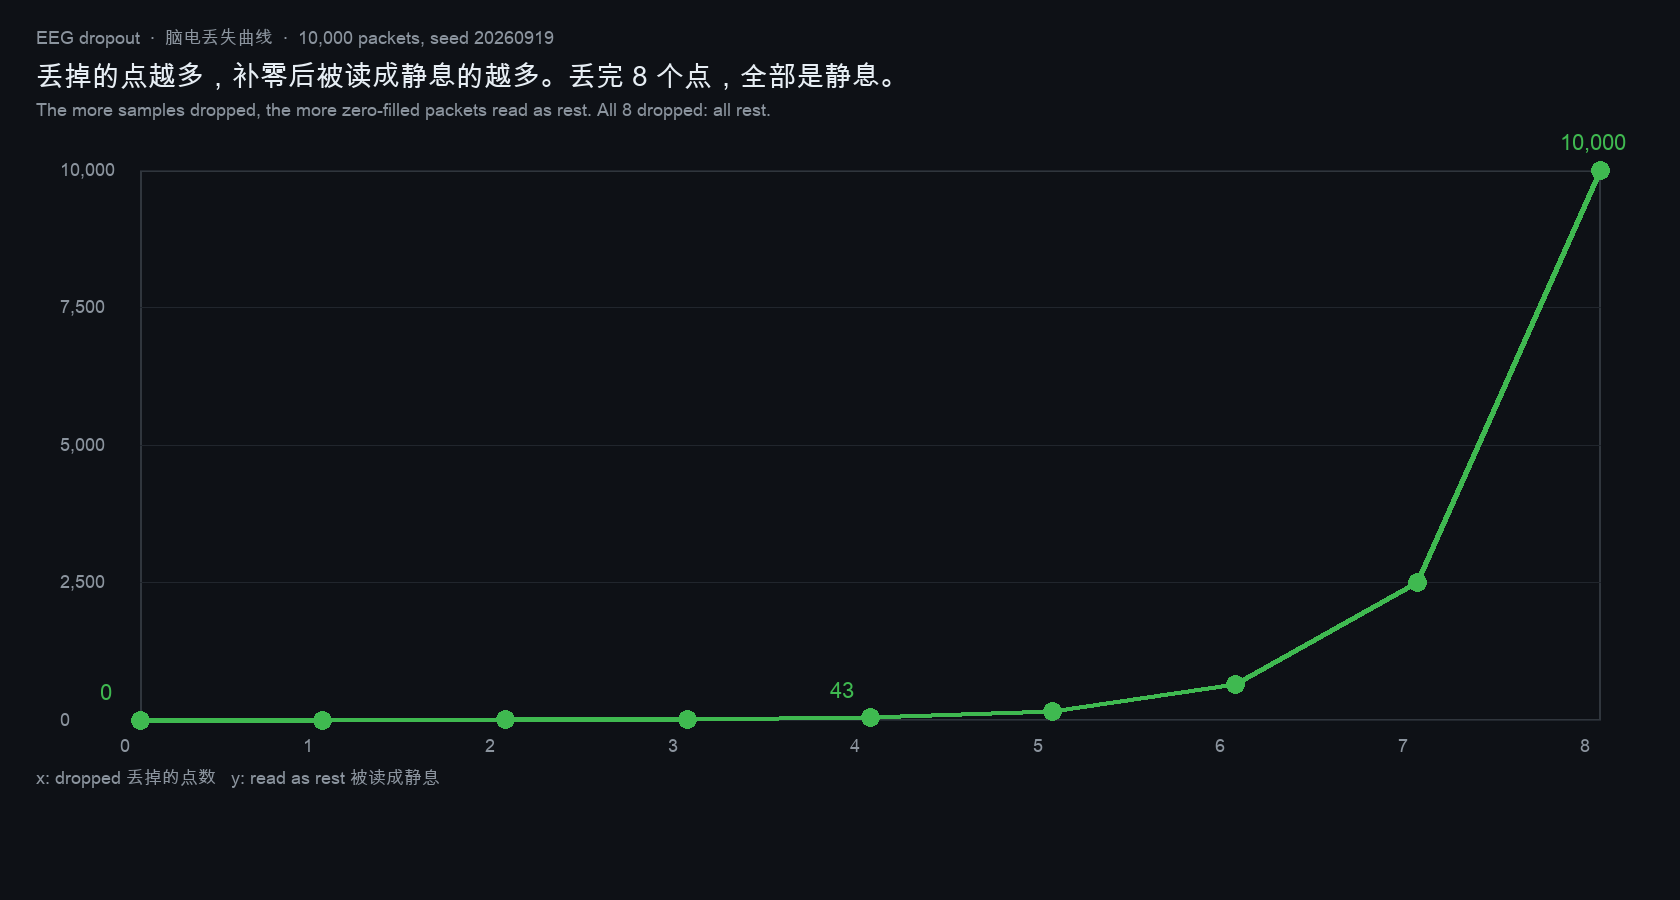
\includegraphics[width=\linewidth]{../../docs/figures/bcisweep.png}
  \caption{EEG packets classified as rest after a suffix of length $k$ is replaced by zeros. Ten thousand packets, eight samples, seed 20260919.}
  \label{fig:eeg}
\end{figure}

\subsection{Two-dimensional grids}
\label{sec:selector}

Each trial is a $16{\times}16$ occupancy grid, obstacle rate $0.15$, mask rate $0.25$, start at the top-left corner and goal at the bottom-right.
A shortest path is computed by breadth-first search.
Optimistic search treats masked cells as free.
Pessimistic search treats them as blocked.

Over 2{,}000 trials the optimistic path crashes 1{,}439 times, stops 61 times, and reaches the goal 500 times, at mean length $30.0$.
The pessimistic path crashes $0$ times, stops 1{,}581 times, and reaches 419 times, at mean length $31.9$.
Figure~\ref{fig:grid} shows one trial in which the optimistic path crosses a masked obstacle.

\begin{figure}[t]
  \centering
  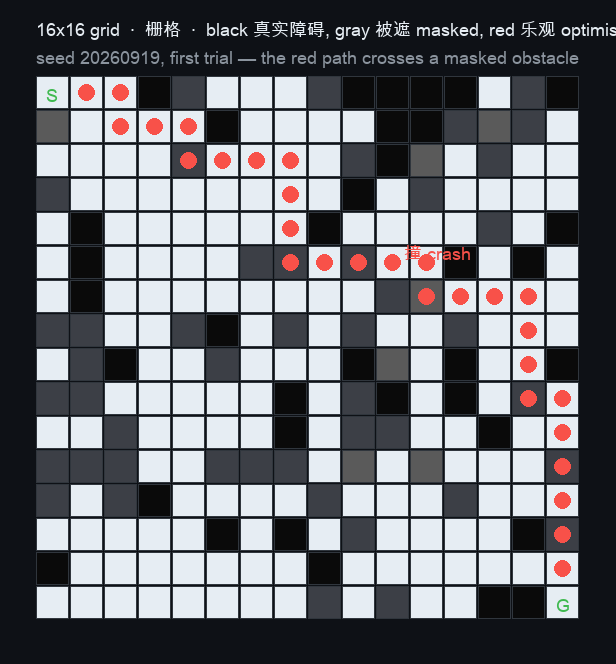
\includegraphics[width=0.92\linewidth]{../../docs/figures/grid2d-map.png}
  \caption{One $16{\times}16$ trial. Black cells are obstacles. Gray cells are masked. The red path is the shortest path after writing masked cells free, and it crosses a masked obstacle.}
  \label{fig:grid}
\end{figure}

\subsection{The selector gap}
\label{sec:selectorgap}

The two paths above are a candidate set.
The visual selector keeps the shorter path, which is the quantity a completed map exposes.
The oracle keeps a path that does not cross a true obstacle, if one exists.

On the same 2{,}000 grids the visual selector reaches 500 times and crashes 1{,}439 times.
The oracle reaches 797 times.
The gap is 297 reached trials (Figure~\ref{fig:selector}).
Those 297 successes are already in the candidate set.
The visual score does not select them.
This is the selection gap reported as robot success in~\cite{visual2026}, measured here as a count.
The $68.9\%$ and $79.2\%$ figures from that paper are not reproduced, because those rollouts are not rerun.

\begin{figure}[t]
  \centering
  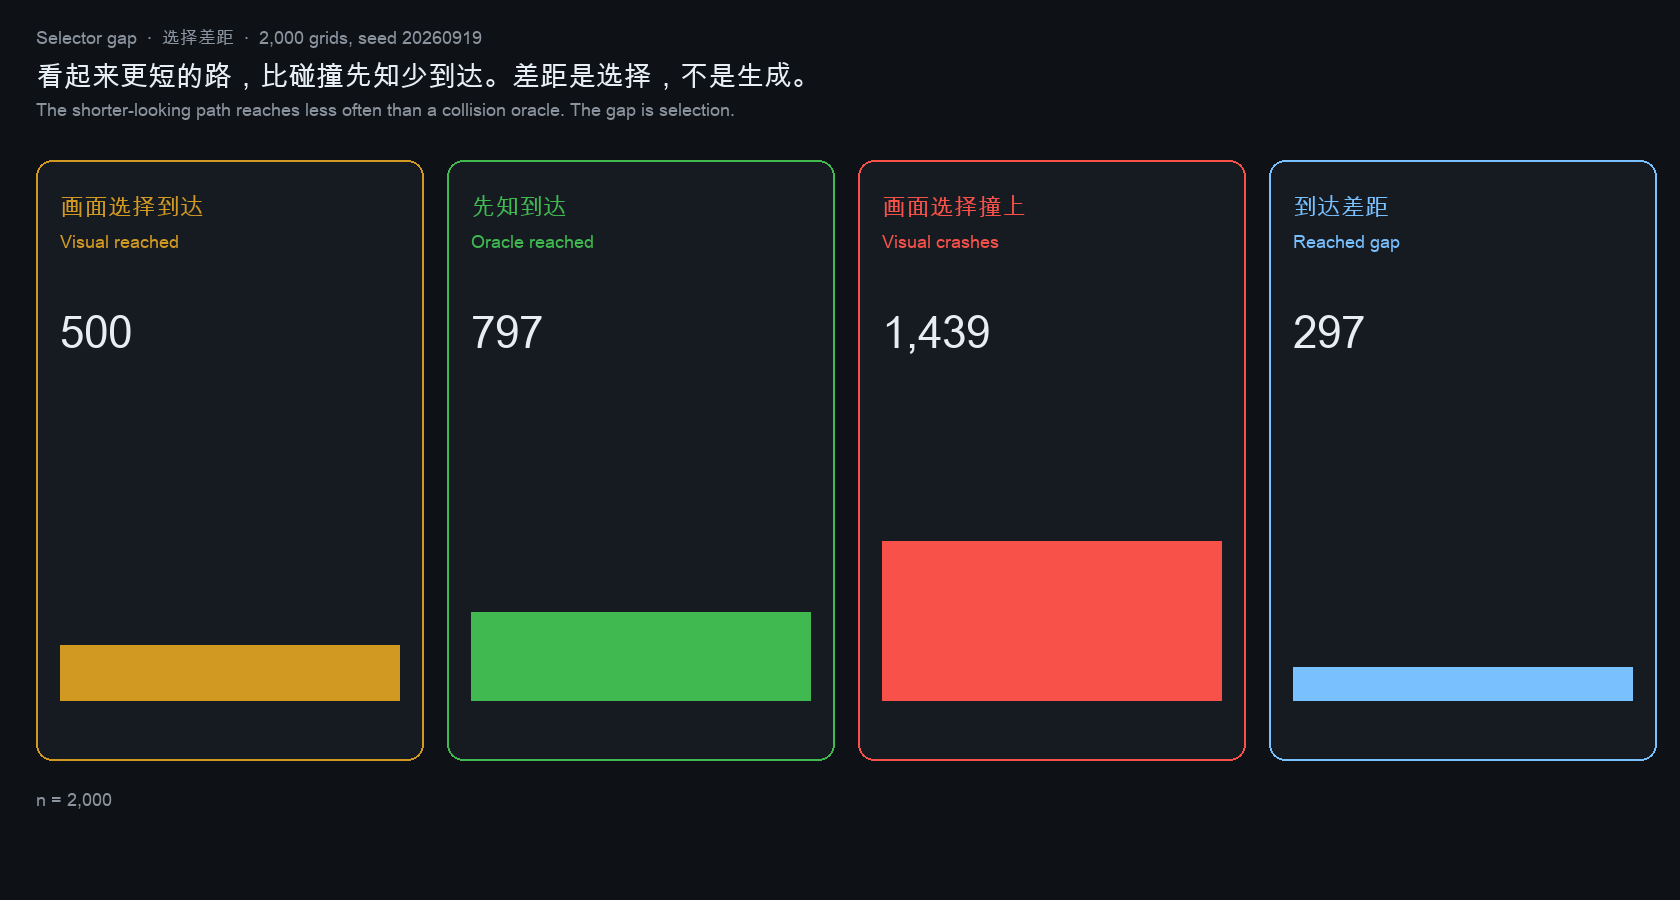
\includegraphics[width=\linewidth]{../../docs/figures/selector.png}
  \caption{Selection on 2{,}000 grids. The shorter imagined path reaches 500 times. An oracle over the same two plans reaches 797 times.}
  \label{fig:selector}
\end{figure}

\subsection{Audit and intervals}

Imputed maps contain $0$ mask markers by Theorem~\ref{sec:ops}'s construction, checked on all 10{,}000 corridors.
A checker that looks for a missing-data flag therefore catches none of the 8{,}564 maps that still hide an obstacle.
Only 1{,}436 imputed maps match the true corridor cell for cell.

Wilson $95\%$ intervals on the pinned rates are narrow.
Occluded corridors: $0.8564$ with interval $[0.8494,0.8631]$.
Optimistic entry: $0.2995$ $[0.2906,0.3086]$.
One-step collision: $0.0552$ $[0.0509,0.0598]$.
Exact map match: $0.1436$ $[0.1369,0.1506]$.
Closed-loop completion of the corridor: $0.0009$ $[0.0005,0.0017]$.

Five seeds at 2{,}000 corridors and mask rate $0.30$ move the completion counts (sweep entries $605,641,580,606,560$; one-step crashes $120,143,127,126,105$) and leave every measured-side column at $0$.

\subsection{Upstream behavior on empty input}

The empty-input result is not special to our generators.
MuJoCo 3.13.0 loads an empty model.
The Munkres implementation 1.1.4 returns an empty list for an empty cost table.
NumPy reports a norm of $0.0$ and a mean of NaN.
MNE-Python 1.9.0 reports duration $0$.
NetworkX reports $0$ nodes.
FilterPy accepts an empty update and leaves the state at $0.0$.
An empty MCAP log and an empty rosbag2 folder contain no messages.
On each of these inputs the corresponding operator here raises, while the occupied input keeps the value cited above.

\subsection{Horizon, discount, and mask rate}
\label{sec:curves}

Figure~\ref{fig:horizon} is the pinned 256-node world.
Reach after one step is $24$.
The fixed point is $214$, met at horizon $12$ and unchanged through horizon $256$.
A single call to the fixed-point operator returns $214$.
The walk is therefore not an approximation that never arrives.
It arrives, and the index is $12$.
Median time per call on the reference machine grows with the horizon and flattens at the same index.
A fixed-point call is about $0.09$\,ms.
The times are reported, not pinned.

\begin{figure}[t]
  \centering
  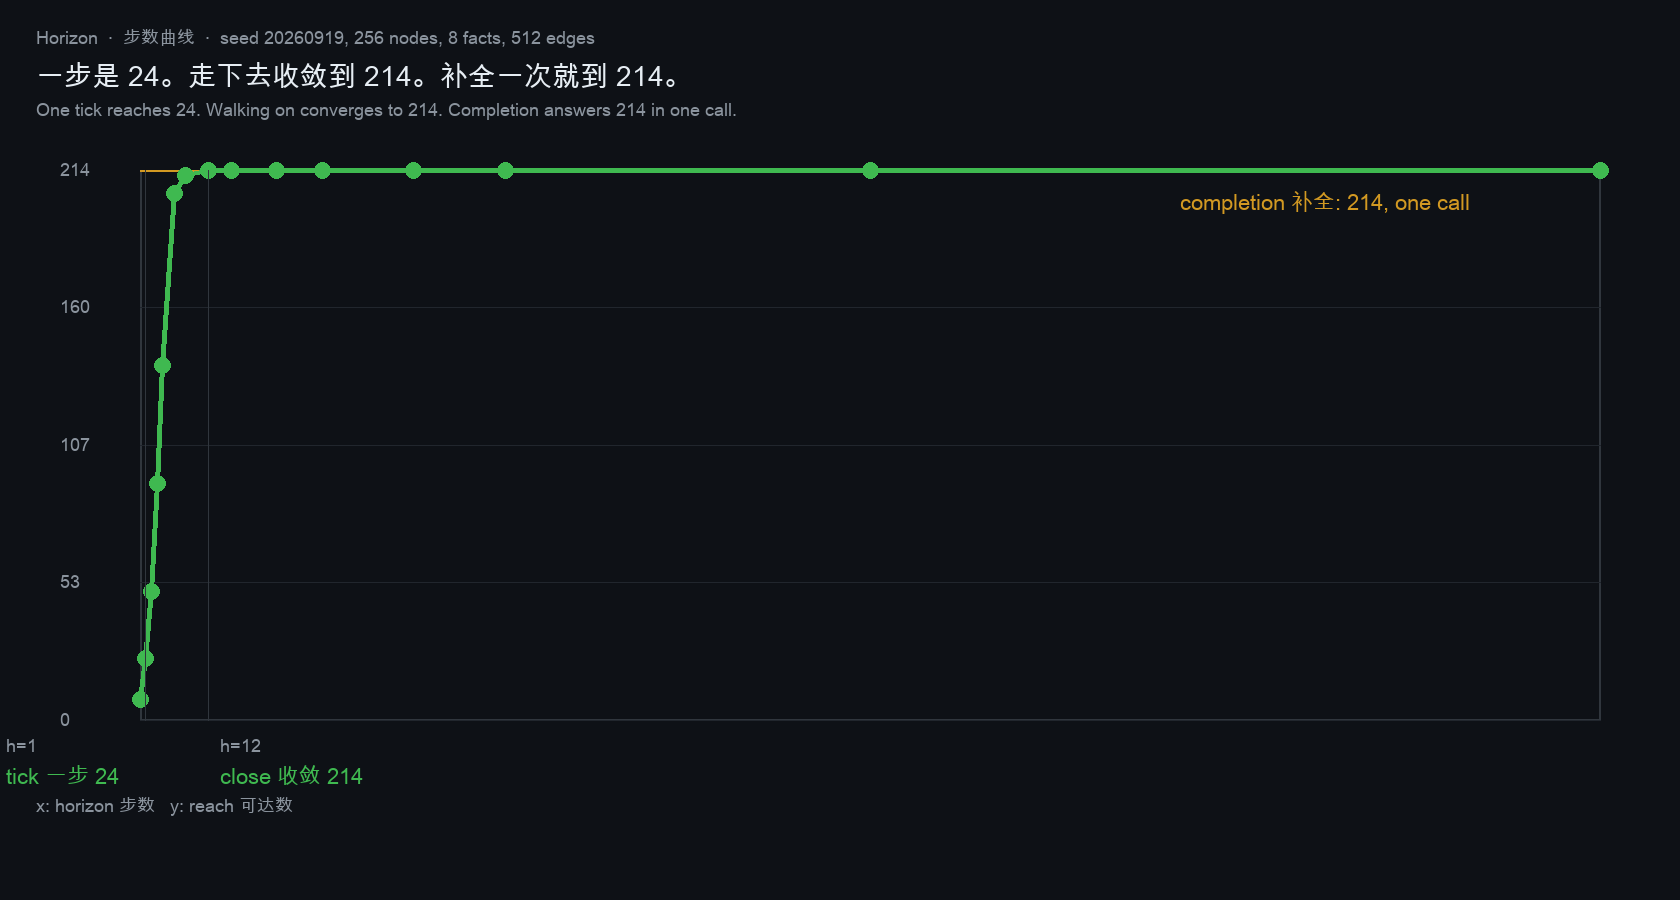
\includegraphics[width=\linewidth]{../../docs/figures/horizon.png}
  \caption{Reach versus horizon on the pinned world. One step is $24$. The fixed point $214$ is met at $12$ steps. Imputation returns $214$ in one call.}
  \label{fig:horizon}
\end{figure}

Figure~\ref{fig:foresight} checks Theorem~1 on a discount grid and on random traps.
Below $9/101$ the trap selects action $0$.
Above it, action $1$.
All $1{,}000$ random traps flip between discount $0$ and discount $0.9$.
Combined with the depth result, the picture is: the flip is a property of one backup, not of a long unroll, once the discount has crossed the threshold.

\begin{figure}[t]
  \centering
  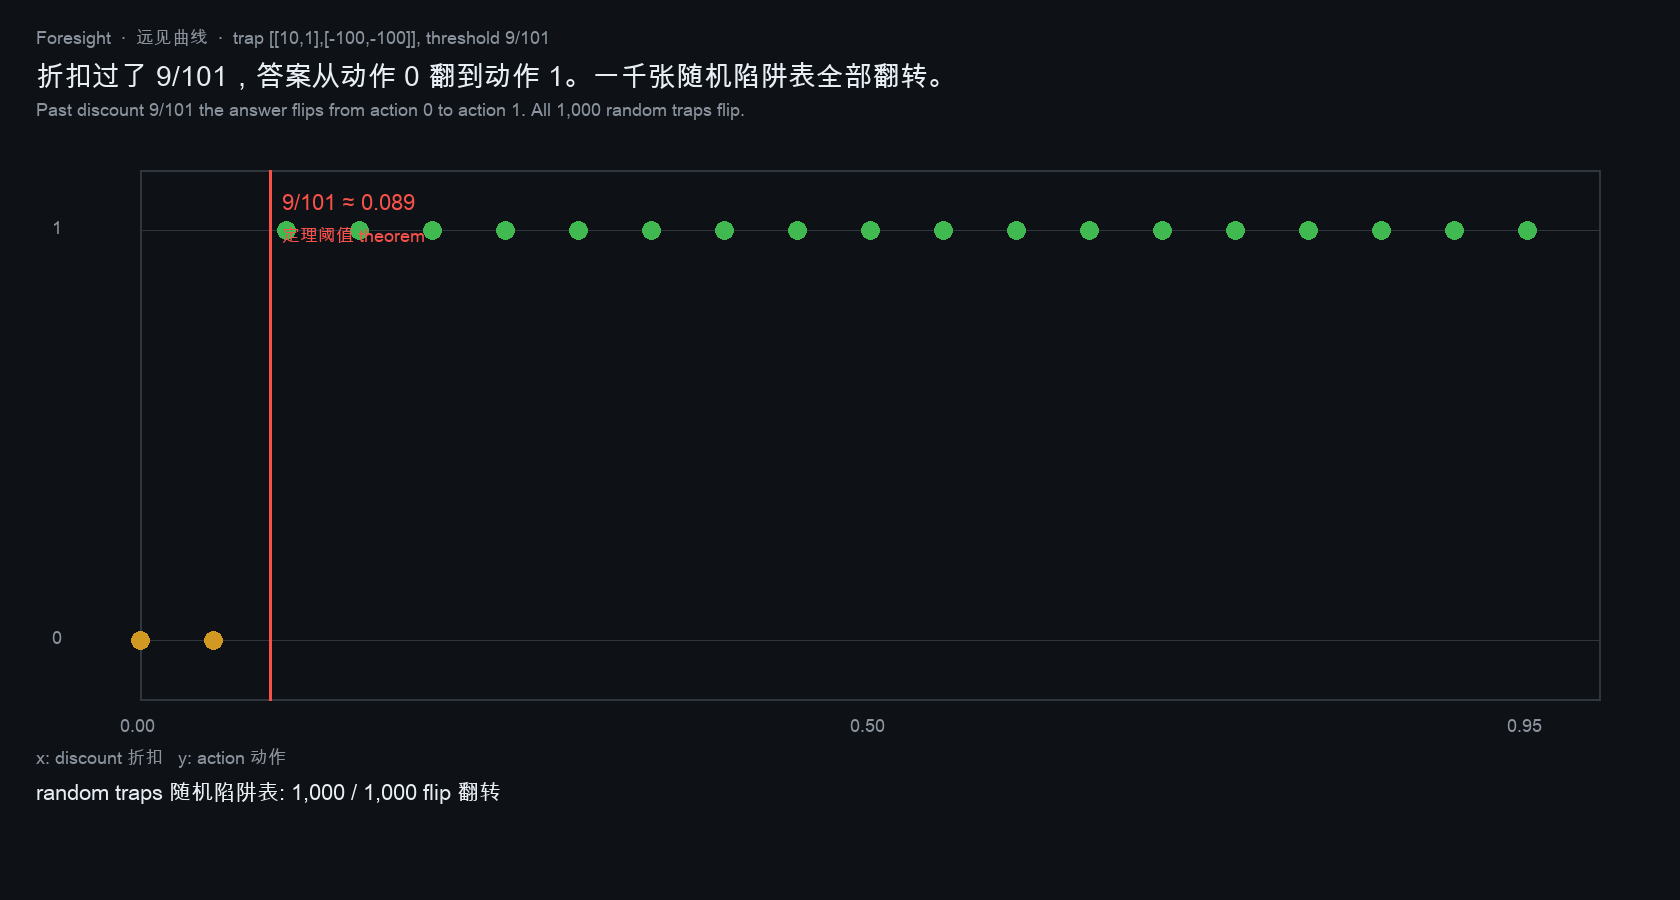
\includegraphics[width=\linewidth]{../../docs/figures/foresight.png}
  \caption{Optimal action on the trap versus discount. The vertical line is the closed-form threshold $9/101$.}
  \label{fig:foresight}
\end{figure}

Figure~\ref{fig:sweep} varies only the mask rate, from $0$ to $0.50$, with $10{,}000$ corridors at each rate.
Imputation entries rise monotonically: $0,503,934,2002,2914,3970,5084$.
The measured step remains $0$.
The collision count is therefore a dose of missingness, not a constant of the planner.

\begin{figure}[t]
  \centering
  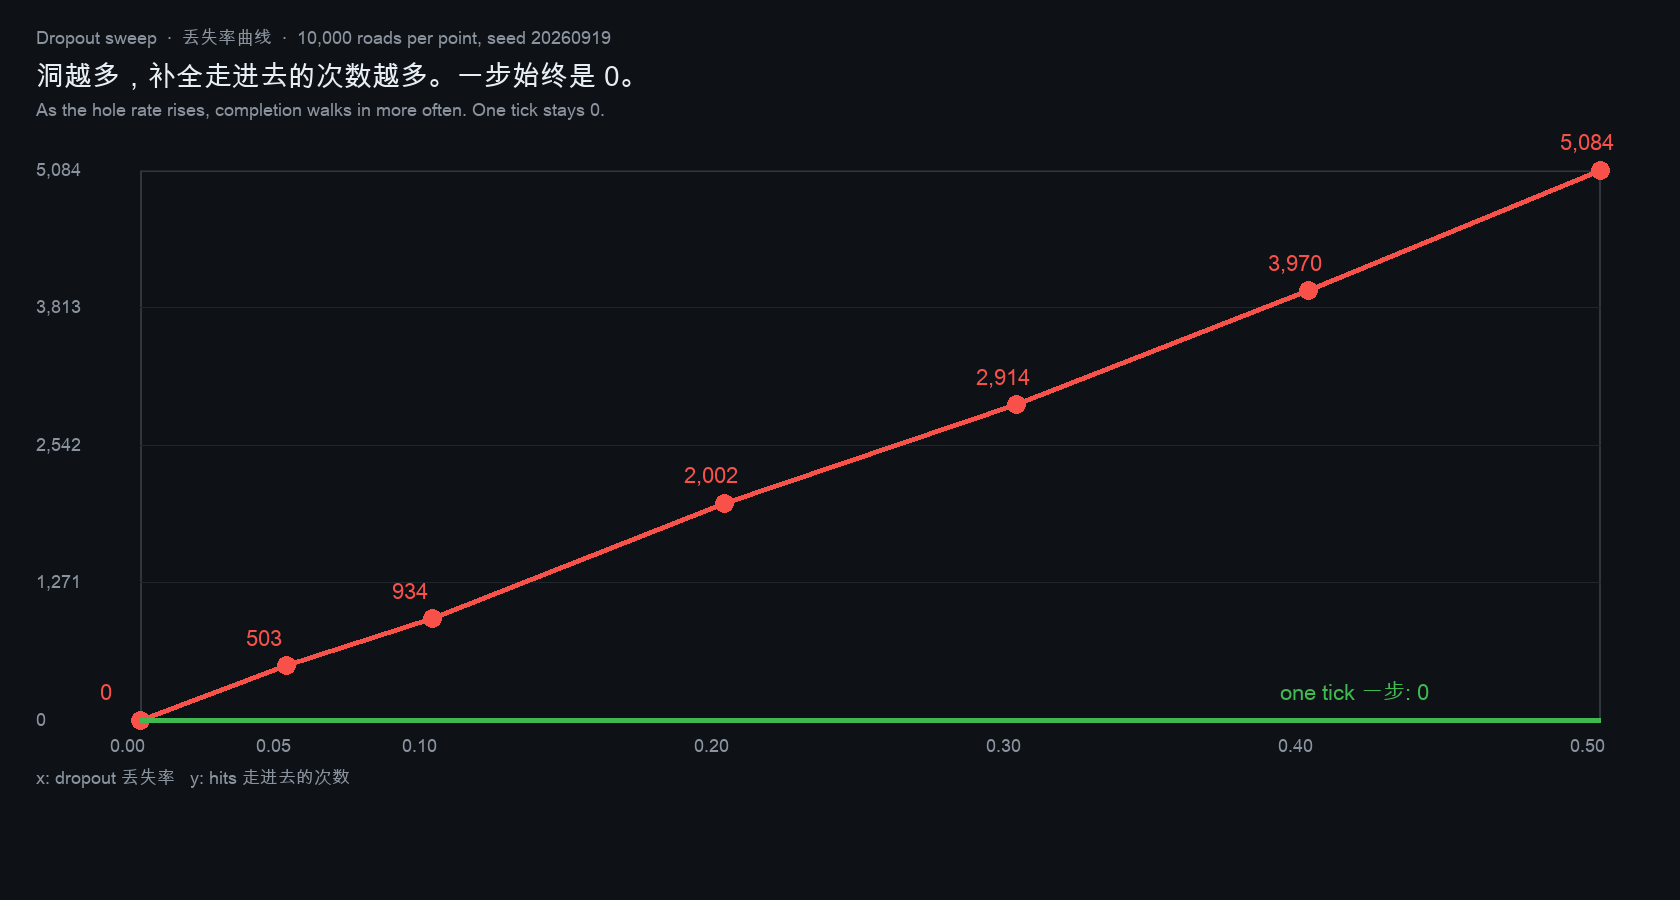
\includegraphics[width=\linewidth]{../../docs/figures/sweep.png}
  \caption{Imputation entries versus mask rate. Each point is $10{,}000$ corridors. The measured step is the flat line at $0$.}
  \label{fig:sweep}
\end{figure}

\subsection{What is pinned}

Table~\ref{tab:pin} collects the counts a reviewer can recompute.
Seeds, widths, and rates are arguments of the scripts named in the repository.
A checker compares every integer in the technical report with the JSON those scripts write.
This manuscript uses the same JSON.

\begin{table}[t]
  \centering
  \small
  \setlength{\tabcolsep}{3pt}
  \begin{tabular}{lrr}
    \toprule
    Quantity & Impute & Measure \\
    \midrule
    3-cell reach & 3 & 2 \\
    8-cell reach (10k) & 8 & 2 \\
    EEG class, filled vs recorded & 0 & 1 \\
    Trap action, row vs backup & 0 & 1 \\
    Occluded corridors / 10k & \multicolumn{2}{c}{8{,}564} \\
    Entries into an occluded obstacle & 2{,}995 & 0 \\
    Next-cell collisions & 552 & 0 \\
    Stops on a free next cell & 0 & 2{,}353 \\
    Full walks, opt.\ vs pes. & 12 & 0 \\
    $16{\times}16$ crashes / reached & 1{,}439 / 500 & 0 / 419 \\
    Selector reached, visual / oracle & 500 & 797 \\
    Closed-loop crashes / waits & \multicolumn{2}{c}{0 / 20{,}975} \\
    \bottomrule
  \end{tabular}
  \caption{Pinned counts. The right column is the measured step or the pessimistic plan, except the last row, which is the closed loop.}
  \label{tab:pin}
\end{table}

\section{What the integers say}

The counterintuitive fact is numerical, not rhetorical.
After optimistic imputation, reachability on a masked chain equals reachability on a chain that was fully observed.
A zero-filled EEG packet is classified as rest, which is the class of a packet that really was zero.
The shorter path on a completed grid is the path that crosses masked obstacles.
In each case the imputed integer is a legal output of the downstream algorithm.
It is the same integer the algorithm returns when the missing part was truly free, truly silent, or truly short.
The measured step returns a different integer, or raises.

The 2026 papers already separate visual quality from the decision~\cite{nilaksh2026,visual2026}.
The experiments here show that the separation survives after the generator is removed.
No network is trained.
The fill is a deterministic write.
The write is sufficient to produce the collision, the class error, and the selector gap.

The write is sufficient to produce the collision, the class error, and the selector gap.

\section{Comparison with the published gap}

Table~\ref{tab:cmp} places our counts next to the published statements they correspond to.
The correspondence is the operator, not the benchmark.
Nilaksh~\etal compare latent spaces by image metrics and by policy return, and find the rankings differ~\cite{nilaksh2026}.
Our analogue is the pair (imputed reach, measured reach): $8$ versus $2$ on every one of 10{,}000 chains, and $3$ versus $2$ on the three-cell chain.
The imputed map is the one a reconstruction loss would accept, because every cell has a value.
The measured step is the one that still knows which cells were missing.

The test-time planning study reports an oracle gap of $79.2-68.9=10.3$ percentage points on robot success~\cite{visual2026}.
Our analogue, on 2{,}000 grids, is $797-500=297$ reached trials, which is $14.9$ percentage points of the trial set.
The visual policy is not a weak generator.
It is the shortest path on the imputed grid, and it is exactly the optimistic row of Section~\ref{sec:selector}: 500 reached and 1{,}439 crashes.
The oracle's extra 297 trials are pessimistic paths that the length score ranks second.
World-coherent decoding argues that the future one selects changes the action~\cite{wcd2026}.
Here the future is one bit per masked cell, and changing that bit from free to wall changes the crash count from 1{,}439 to $0$ and the reached count from 500 to 419.

\begin{table}[t]
  \centering
  \small
  \setlength{\tabcolsep}{3pt}
  \begin{tabular}{p{0.42\linewidth}p{0.48\linewidth}}
    \toprule
    Published statement & Count in this paper \\
    \midrule
    Pixel match need not be the planning ranking~\cite{nilaksh2026} &
    Imputed reach equals the fully observed reach ($3{=}3$, and $8{=}8$ on 10k chains) while one step is $2$ \\
    Visual selectors leave an oracle gap~\cite{visual2026} &
    Shorter path reaches 500; oracle over the same plans reaches 797 \\
    Masked EEG is predicted or interpolated~\cite{jiang2024labram} &
    A fully zero-filled go packet is class 0 on 10{,}000 / 10{,}000 trials \\
    \bottomrule
  \end{tabular}
  \caption{The published claim and the integer that corresponds to it. Robot percentages from those papers are not re-estimated.}
  \label{tab:cmp}
\end{table}

Figure~\ref{fig:stats} is the uncertainty on the headline rates.
The intervals are Wilson intervals at $z=1.96$ applied to the pinned counts, not a bootstrap and not a second draw.
The one-step collision rate $0.0552$ has interval $[0.0509,0.0598]$.
The occluded-corridor rate $0.8564$ has interval $[0.8494,0.8631]$.
Neither interval contains the measured-step rate, which is $0$.
A reader who wants a larger grid, a real tokenizer, or a robot log can change the generator.
The comparison that has to survive that change is the one in the table: the imputed integer, the measured integer, and the selector gap.

\begin{figure}[t]
  \centering
  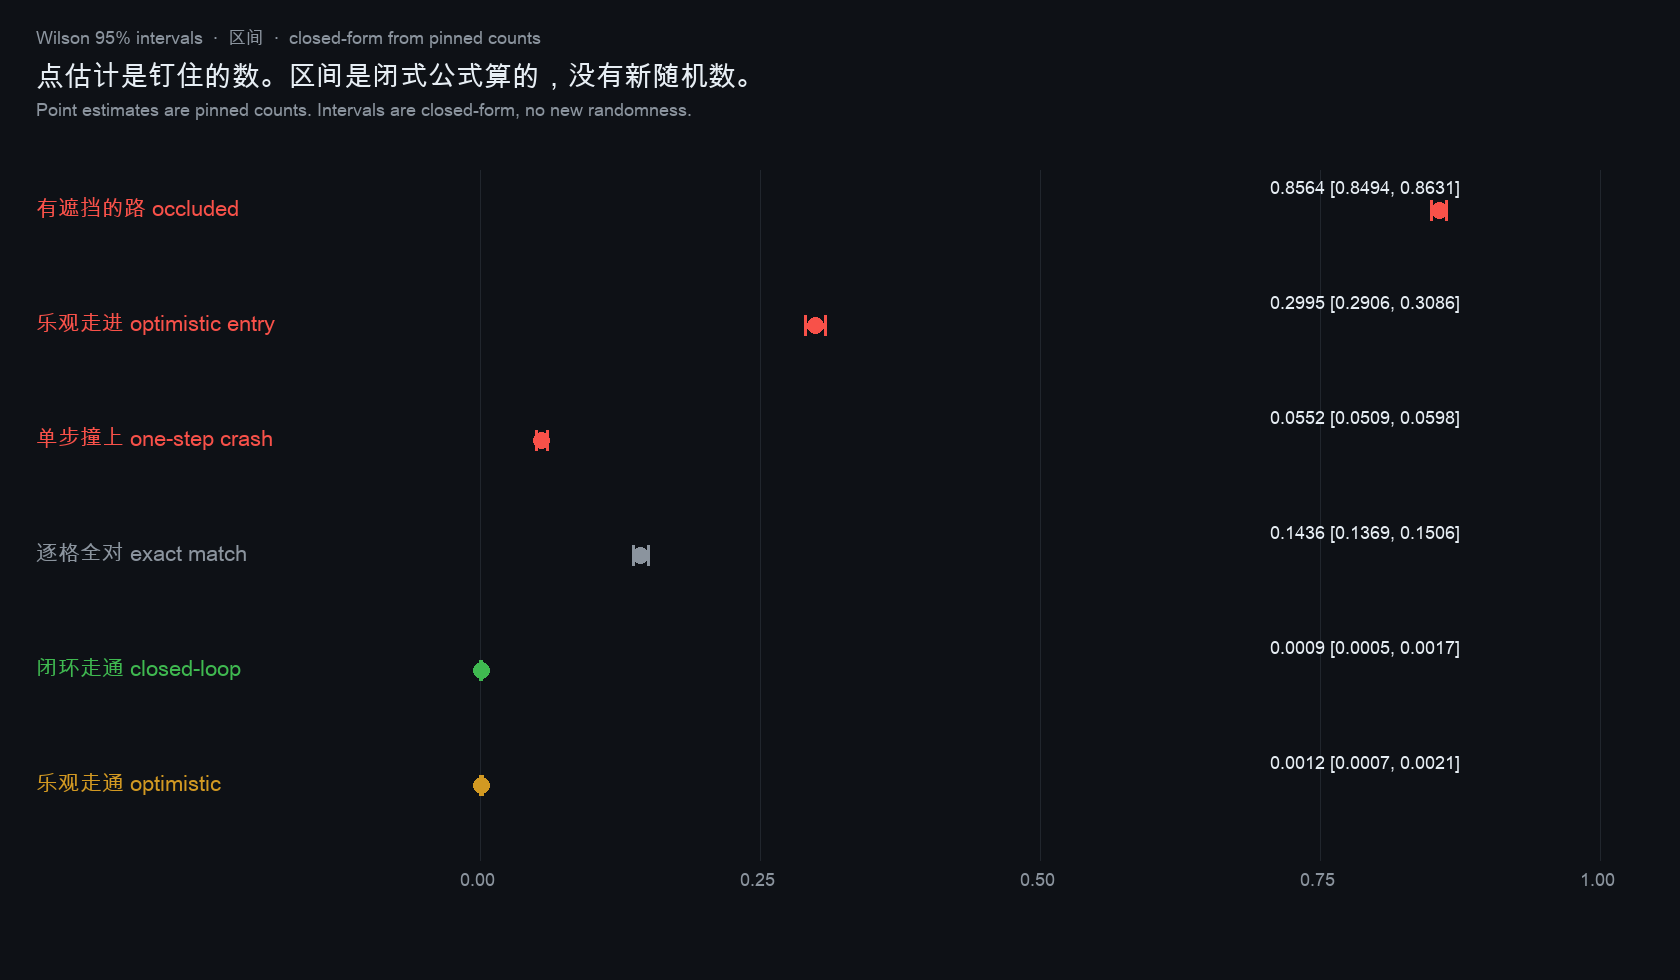
\includegraphics[width=\linewidth]{../../docs/figures/stats.png}
  \caption{Wilson $95\%$ intervals on pinned rates. The measured-step collision rate is $0$ and is not drawn.}
  \label{fig:stats}
\end{figure}

\section{Reproducibility}

Every integer in Section~\ref{sec:exp} is an argument of a script and a field of a JSON file.
The manuscript is checked by comparing those fields to the tokens in the technical report.
The check is part of the continuous build.
Seeds are 20260919 unless a range is named.
Obstacle rates, mask rates, widths, and depths are constants at the top of each script.
Policy evaluation and finite-horizon backups use exact rationals, so the discount threshold does not depend on a floating-point tolerance.
What is deliberately not pinned is wall-clock time.

\section{Empty input, side by side}
\label{sec:empty}

The fail-closed behavior is checked against the libraries that already return a number on empty input.
MuJoCo 3.13.0 loads an empty model.
Munkres 1.1.4 returns an empty list on an empty cost table.
NumPy reports a norm of $0.0$ and a mean of NaN.
MNE-Python 1.9.0 reports duration $0$ and zero annotations.
NetworkX reports zero nodes on an empty digraph.
FilterPy accepts an empty update and leaves the state at $0.0$.
An empty MCAP log and an empty rosbag2 folder contain no messages.
On each of these inputs the operator in this paper raises.
On the occupied input the value is unchanged: assignment cost $2$, letter distance $3$ on \texttt{CAKE}, eight EEG samples with markers go and end, one lidar pair counted as $1$, three observations counted as $3$, and a three-node chain whose one-step reach is $2$ and whose fixed point is $3$.

Figure~\ref{fig:cost} is why the fixed point is not free.
On the 256-node world the reach curve and the per-call time flatten together at horizon $12$.
Returning $214$ by imputation is one call, about $0.09$\,ms on the reference machine.
Walking the twelve steps costs more than that call and returns the same integer only at the end.
Before horizon $12$ the two answers differ, which is the entire content of the horizon plot.

\begin{figure}[t]
  \centering
  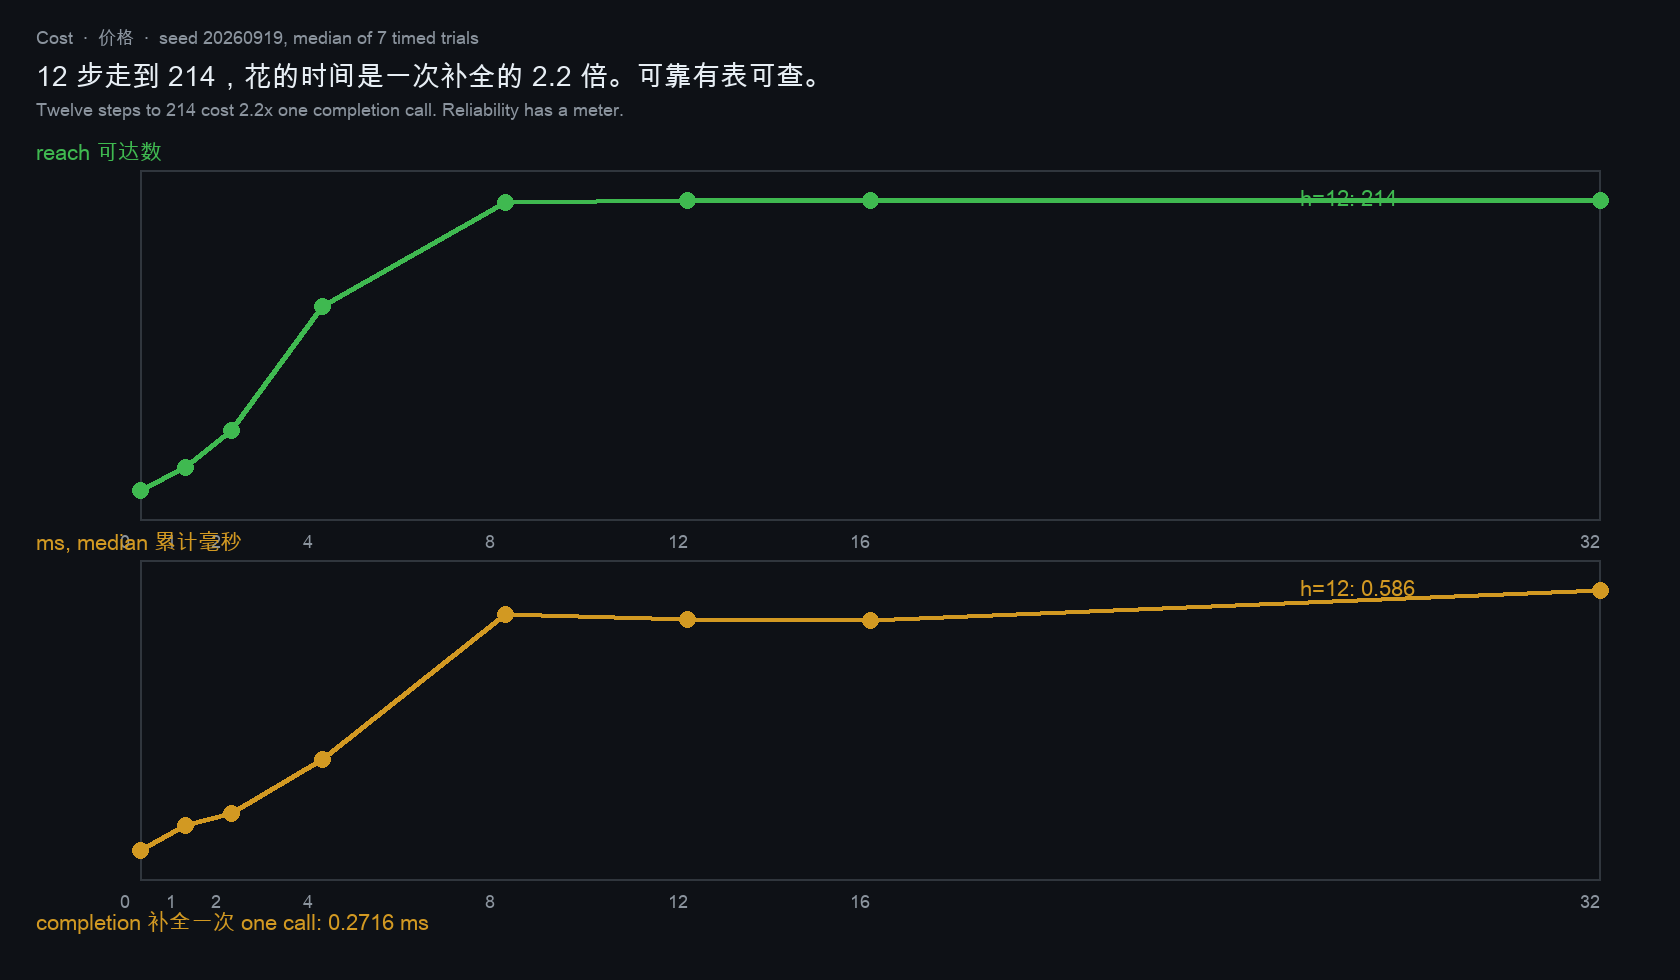
\includegraphics[width=\linewidth]{../../docs/figures/cost.png}
  \caption{Reach and per-call time versus horizon. Both flatten at $12$ steps. The fixed-point call is one point, not a curve.}
  \label{fig:cost}
\end{figure}

\section{Worked algebra}

The threshold in Theorem~1 is the comparison of two stationary policies, not a numerical search.
Write the reward of action $a$ in state $s$ as $r(s,a)$, with
\[
r(0,0)=10,\quad r(0,1)=1,\quad r(1,0)=r(1,1)=-100.
\]
The transition is deterministic, $s'= (s+a+1)\bmod 2$.
Action $0$ therefore swaps the two states.
Action $1$ stays.

Under the policy that always takes action $0$,
\begin{align}
V_0 &= 10 + d V_1, \\
V_1 &= -100 + d V_0.
\end{align}
Substitute $V_1$ into the first line:
\[
V_0 = 10 + d(-100 + d V_0) = 10 - 100d + d^2 V_0,
\]
and for $d\in[0,1)$,
\[
V_0 = \frac{10-100d}{1-d^2}.
\]
A one-step deviation to action $1$ in state $0$ collects $1$ and returns to state $0$, so its action value against the same continuation is $1+dV_0$.
The deviation is profitable exactly when
\begin{align}
1 + d V_0 &> V_0 \\
1 &> V_0(1-d) \\
1 &> \frac{10-100d}{1+d},
\end{align}
where the last step uses $1-d^2=(1-d)(1+d)$ and $1-d>0$.
Clearing the positive denominator yields $1+d > 10-100d$, hence $101d>9$, hence $d>9/101$.
At $d=9/101$ the two action values are equal.
The implementation breaks ties toward the lower action index, so the reported flip is the first grid point strictly above the threshold.
The hundredths grid therefore stays on action $0$ through $0.08$ and is on action $1$ from $0.09$ onward.
The plotted curve uses steps of $0.05$, so the first drawn flip is $0.10$, which is the first plotted point above $9/101$.

The same linear system is what policy evaluation solves.
$(I-dP)$ is singular at $d=1$ because $P$ is a permutation matrix, so the grid stops at $0.95$.
Integer scaling of the same Bellman update does not preserve the threshold: the discounted continuation grows without a common denominator, and the argmax flips early.
Exact rationals are the evaluation used for the curve and for the $1{,}000$ random traps, all of which flip between the myopic action and the one-step action at a positive discount.

Finite horizon has a separate off-by-one.
Depth $0$ returns the argmax of the raw row, which is action $0$ on this trap.
Depth $1$ performs one backup of the continuation and then the same argmax, which is already action $1$ at discount $9/10$.
Further backups do not change the action.
The curve of selected actions against depth is therefore $0,1,1,1,1,1$.
An implementation that counts the raw row as a backup reports the flip one step late.

Reachability has the same shape without a discount.
Let $R_h$ be the set of nodes reachable in at most $h$ steps from the observed facts, using only observed edges.
Then $R_h\subseteq R_{h+1}\subseteq R_\infty$, so the cardinalities are nondecreasing and bounded, and they stabilize at the least fixed point of the completion operator.
On the pinned world that sequence is $8,24,50,92,138,205,212,214$, and $214$ is also the integer returned by one call to the completion operator.
Any horizon short of $12$ is a different integer.
Imputation that returns $214$ is therefore claiming the walk has already finished.

The closed loop makes the same distinction in time.
On 10{,}000 corridors it records $0$ crashes, $9$ goals, $9{,}991$ correct stops, and $20{,}975$ waits, with a cap of $2{,}000$ waits per trial and $0$ timeouts.
A wait is a re-observation, not a motion.
Dividing waits by the open-loop crash count gives the breakeven in Theorem~5: $20975/2995$ lies in $(7.0, 7.1)$.
One-step decisions use a different pair, $2353$ extra stops against $552$ crashes, so the breakeven is the reduced fraction $2353/552$, which lies in $(4.2, 4.3)$.
The two ratios answer different questions.
The one-step ratio prices a single decision.
The walk ratio prices a trajectory that may wait many times before the mask clears.
Neither ratio is a learned cost.
Both are counts.

Across five seeds the completion side moves and the measured side does not.
At mask rate $0.30$ and $2{,}000$ corridors per seed, the completion hits are $605,641,580,606,560$ and the one-step crashes are $120,143,127,126,105$.
Every measured-step column in that table is $0$.
The variance is in how often the mask covers an obstacle, which changes with the seed.
It is not in the rule that refuses to enter a masked cell.

The selector gap has the same source and a different score.
On the $16{\times}16$ grids the optimistic shortest path reaches the corner on 500 of 2{,}000 trials and crashes on 1{,}439.
The pessimistic shortest path crashes on none and reaches on 419.
A length score that prefers the shorter of the two existing paths selects the optimistic path whenever both exist and the optimistic path is no longer, which is the usual case: writing masked cells free can only shorten a path.
The visual policy is therefore identical to the optimistic row, 500 reached and 1{,}439 crashes.
An oracle that accepts a plan when either path reaches, and that knows which path collides, adds the 297 pessimistic successes the length score ranked second.
The gap is $797-500$.
It is not a property of a neural ranker.
It is the property that the shorter imagined path is the one that was allowed to cross a cell nobody observed.

A follow-up that attaches the same audit to a learned world model has a narrow measurement to report.
Take a public video or robot log, mask a known subset of the observation, and run the model's own imputer.
Then score two maps with the same planner: the map the imputer returned, and the map that still carries the mask.
The three integers to publish are the imputed outcome, the masked outcome, and the selector gap between a visual score and a collision oracle on that pair of plans.
If those three integers move together when the generator changes, the fill is not the carrier of the risk.
If they separate the way they separate here, the fill is.
That experiment is not in this paper.
The generators here are the deterministic writes named above, and the integers are the ones in Table~\ref{tab:pin}.

\section{Limitations}

Corridors are one-dimensional, and the grids are $16{\times}16$ with a point start and goal.
The EEG rule is a sum threshold, not LaBraM's tokenizer.
The traps are two states.
Robot success rates from the cited papers are not re-run, and no claim is made about them.
Timings are from one machine and are not pinned.
The positive claim is the one the integers support: optimistic imputation decides the failure mode, a measured step does not enter unobserved cells, and a visual score over the resulting plans leaves an oracle gap of 297 reached trials out of 2{,}000.

\section{Conclusion}

Imputation writes a usable value into unobserved input.
On the distributions in this paper that value matches a fully observed world often enough to be planned on, and often enough to be wrong.
A measured transition, a pessimistic fill, and a closed loop that re-observes before moving do not cross occluded obstacles.
Selecting the plan by how short it looks on the imputed map misses 297 goals that a collision oracle finds in the same candidate set.
The discount at which lookahead flips the trap is $9/101$, and one backup is enough for the one-step family.
The counts are in the repository and are checked against this text on every build.

{
\small
\bibliographystyle{ieeenat_fullname}
\bibliography{main}
}

\end{document}
